\documentclass{article}

% NeurIPS-style author/year papers commonly use natbib and a tight style.
% If you later switch to the official neurips_20xx class, these sections
% should still compile with minimal changes.
\usepackage[final]{neurips_2024}

\usepackage[utf8]{inputenc}
\usepackage[T1]{fontenc}

\usepackage{amsmath,amssymb,amsthm}
\usepackage{mathtools}
\usepackage{microtype}
\usepackage{booktabs}
% \usepackage{algorithm}
% \usepackage{algpseudocode}
\usepackage{graphicx}
\usepackage{multirow}
\usepackage{hyperref}
\usepackage{cleveref}
\usepackage{xcolor}

\crefname{equation}{equation}{equations}
\Crefname{equation}{Equation}{Equations}
% natbib is already loaded by neurips_2024; avoid option clashes. 

% -------------------- theorem environments --------------------
\newtheorem{theorem}{Theorem}
\newtheorem{proposition}{Proposition}
\newtheorem{lemma}{Lemma}
\newtheorem{definition}{Definition}

% -------------------- macros --------------------
\newcommand{\cD}{\mathcal{D}}
\newcommand{\cS}{\mathcal{S}}
\newcommand{\cT}{\mathcal{T}}
\newcommand{\E}{\mathbb{E}}
\newcommand{\R}{\mathbb{R}}
\newcommand{\X}{\mathbf{X}}
\newcommand{\x}{\mathbf{x}}
\newcommand{\alphab}{\boldsymbol{\alpha}}
\newcommand{\onevec}{\mathbf{1}}
\newcommand{\K}{\mathbf{K}}
% \odot and \oslash are standard math symbols; do not redefine them.

\title{Stable and Efficient Exact Shapley Values for Product Games via Gauss--Legendre Quadrature}

\author{Anonymous Authors}

\begin{document}
\maketitle

\begin{abstract}
We study the exact computation of Shapley values for \emph{product games} — cooperative games in which the coalition value factorizes as a product of per-player terms. Such games arise in machine learning explainability whenever the underlying value function inherits a multiplicative structure from the model, as in kernel methods with product kernels and tree-based models evaluated along individual decision paths. Our central observation is that, for a product game, the Shapley value of each player admits an exact one-dimensional integral representation: the exponential weighted sum over feature coalitions collapses to the integral of a degree-$(d-1)$ polynomial over $[0,1]$, where $d$ denotes the total number of features. This yields a Gauss--Legendre quadrature scheme that is \emph{provably exact} when the number of nodes $m_q$ satisfies $m_q \geq \lceil d/2 \rceil$, and provides a principled approximation with exponentially decaying error otherwise — an approximation regime that is practically highly effective, as we verify empirically across models with thousands of features using only a few hundred nodes. Building on this formulation, we derive a numerically stable implementation via log-space evaluation, and an efficient parallel implementation based on associative scan primitives. Under a parallel execution model, the algorithm achieves $O(d\,m_q)$ total work and $O(\log d)$ parallel time. Applied to tree ensembles, the exact variant matches the complexity of Linear TreeSHAP, while remaining numerically stable, and our benchmarks show it is the fastest exact method across all tested configurations.


% Exact Shapley value computation is generally exponential in the number of features, and even model-specific accelerations can become numerically unstable when the underlying structure involves many variables. We address this problem for a broad class of cooperative games with multiplicative structure, which we call product games. We show that for such games, the Shapley value admits an exact one-dimensional integral representation, transforming the combinatorial weighted sum over subsets into the integral of a polynomial over $[0,1]$. This yields a simple Gauss--Legendre quadrature method that is exact when the quadrature rule matches the polynomial degree and provides a systematic approximation otherwise. Based on this formulation, we further develop a numerically stable algorithm using log-space evaluation, and a parallel implementation based on associative scan primitives. Under a parallel model, the method achieves $O(D\,m_q)$ total work and $O(\log D)$ parallel time, where $D$ denotes the effective dimension of the product structure and $m_q$ is the number of quadrature nodes, both of which are lower than the number of features. The framework covers important explainability settings in machine learning, including kernel methods with product kernels and tree-based models along individual decision paths.
\end{abstract}

%%%%%%%%%%%%%%%%%%%%%%%%%%%%%%%%%%%%%%%%%%%%%%%%%%%
%%%%%% Introduction
%%%%%%%%%%%%%%%%%%%%%%%%%%%%%%%%%%%%%%%%%%%%%%%%%%%
\section{Introduction}

Shapley values are a foundational tool for explaining predictions of machine learning models, providing feature attributions with strong axiomatic guarantees from cooperative game theory \citep{shapley}. Their principled nature has led to widespread adoption across explainable AI, both in model-agnostic methods~\citep{shap, shapiq, polyshap} and in model-specific methods that exploit structural properties of particular model classes, including TreeSHAP for tree ensembles~\citep{treeshap, linear_treeshap}, GPSHAP and variants for Gaussian processes~\citep{gpshap,fgpx_shapley}, and RKHS-SHAP for kernel methods~\citep{rkhs_shap}. This breadth of use has made Shapley-based attribution a central paradigm for interpreting modern machine learning systems.

Despite their broad applicability, exact Shapley values are generally expensive to compute, since the definition involves exponentially many feature coalitions. To overcome this, several model-specific methods exploit structural properties of the model under explanation in order to compute exact Shapley values in polynomial time. One particularly important case arises when the underlying model induces a multiplicative structure in the coalition value function used for Shapley attribution. This connects naturally to \emph{product games}, in which the value of a coalition factorizes across players \citep{cooperative_prodcut_games}. Moreover, since the Shapley value is linear in the value function, the same perspective extends directly to weighted sums of product games. Such multiplicative value functions arise in several important explainability settings, including path-dependent tree-based models~\citep{treeshap, linear_treeshap} and kernel methods with product kernels~\citep{pkex_shapley}.


A common strategy for exploiting multiplicative structure reformulates the Shapley computation in terms of polynomial representations and recovers the required coefficients via interpolation. In tree-based models, recent methods leverage Chebyshev or Fourier interpolation to compute Shapley values in linear time by evaluating the underlying polynomial at carefully chosen nodes~\citep{linear_treeshap, fourier_treeshap}. These approaches are asymptotically optimal, but their numerical stability deteriorates rapidly with the degree of the interpolation polynomial: in tree ensembles the degree is governed by the path length, and in more general multiplicative settings it scales with the number of features, rendering interpolation-based methods unreliable in high dimensions. For product-kernel methods, a more stable alternative based on shared algebraic recursions has been proposed~\citep{pkex_shapley}, but at the cost of substantially more arithmetic operations. The literature thus exposes a persistent trade-off between numerical robustness and computational efficiency, with no existing method offering both.

This paper resolves that trade-off by recasting the exponentially-weighted Shapley sum for a product game as the integral of a single polynomial over $[0,1]$. The representation eliminates both subset enumeration and interpolation-based coefficient recovery, and admits a Gauss--Legendre quadrature scheme that is \emph{exact} whenever the number of nodes $m_q \geq \lceil d/2 \rceil$ and geometrically convergent otherwise; empirically, a few hundred nodes deliver near-machine precision for problems with up to $10{,}000$ features. Two structural properties of the integrand then yield an algorithm that is simultaneously stable and fast: the integrand factorizes across features, so at each quadrature node all $d$ Shapley values share a single length-$d$ product computed once in log-space with explicit sign tracking; and this shared product is an associative reduction, hence amenable to parallel-scan primitives~\citep{blelloch1990prefix}. The resulting estimator attains $O(d\,m_q)$ total work and $O(\log d)$ parallel depth under a standard parallel model. Specialized to tree ensembles, it matches the asymptotic complexity of Linear TreeSHAP while remaining numerically stable, and our benchmarks show it is the fastest \emph{numerically correct} exact method across every tested configuration, outperforming \textsc{shap} by $3$--$5{\times}$ at large ensemble sizes while maintaining additivity residuals at floating-point precision.


%%%%%%%%%%%%%%%%%%%%%%%%%%%%%%%%%%%%%%%%%%%%%%%%%%%
%%%%%% Preliminaries
%%%%%%%%%%%%%%%%%%%%%%%%%%%%%%%%%%%%%%%%%%%%%%%%%%%
\section{Preliminaries}
\label{sec:preliminaries}

\paragraph{Notation}
Let $\cD = \{1,\dots,d\}$ denote the set of $d$ input features and $2^\cD$ its power set.
The training set consists of $n$ samples $\{(\x^{(i)}, y^{(i)})\}_{i=1}^n$, where
$\x^{(i)} \in \mathbb{R}^d$ and $y^{(i)} \in \mathbb{R}$ (or a discrete label set in classification).
We write $\X \in \mathbb{R}^{n \times d}$ for the feature matrix.
For a subset $\cS \subseteq \cD$, $\X_{\cS}$ denotes the restriction of $\X$ to the columns indexed by $\cS$,
and $\x_{\cS}$ the restriction of a vector $\x$ to the same subset.
We use bold lowercase letters for vectors, bold uppercase letters for matrices, calligraphic letters for sets, and capital letters for random variables.
Element-wise multiplication and division are denoted by $\odot$ and $\oslash$, respectively, and expectation by $\E$.
A symmetric positive (semi-)definite kernel function is denoted by $k$, with $k_{\cS}$ indicating its restriction to features in $\cS$.
The corresponding kernel matrices are denoted by $\K$ and $\K_{\cS}$, respectively. Proofs are deferred to Appendix~\ref{apx:proofs}.




\paragraph{Shapley values.}
The Shapley value~\citep{shapley} is a classical solution concept from cooperative game theory and a widely used method for feature attribution in explainable machine learning.
It assigns an importance score to each feature by averaging its marginal contribution over all feature coalitions, with weights determined by coalition size.
Among allocation rules for transferable-utility games, it is uniquely characterized by the axioms of \emph{efficiency}, \emph{symmetry}, the \emph{null-player} property, and \emph{linearity}~\citep{shapley,weber1988probabilistic}, and these axioms have been repeatedly invoked as motivation for Shapley-based attribution in explainable ML~\citep{shap,many_sv}.

Formally, given a value function $v : 2^{\cD} \to \mathbb{R}$ that assigns a scalar contribution to each subset of features,
the Shapley value of feature $j \in \cD$ is defined as
\begin{equation}
\label{eq:shapley_def}
\phi_j(v)
=
\sum_{\cS \subseteq \cD \setminus \{j\}}
\mu(|\cS|)
\bigl( v(\cS \cup \{j\}) - v(\cS) \bigr),
\qquad
\mu(s) = \frac{s!\,(d-s-1)!}{d!}.
\end{equation}
The term $v(\cS \cup \{j\}) - v(\cS)$ is the marginal contribution of feature $j$ to coalition $\cS$.%, and by efficiency $\sum_{j=1}^d \phi_j(v) = v(\cD) - v(\varnothing)$.

~\Cref{eq:shapley_def} is a sum over $2^{d-1}$ coalitions, so exact computation is exponential in $d$ for generic $v$.
Scalable Shapley attribution has therefore developed along two complementary directions: \emph{model-agnostic} approximations such as KernelSHAP and its refinements~\citep{shap,shapiq,polyshap,lime}, and \emph{model-specific} exact algorithms that exploit algebraic or combinatorial structure in $v$~\citep{treeshap,linear_treeshap,fourier_treeshap,fast_tree_shap,q-shap,pkex_shapley,fgpx_shapley,rkhs_shap,gpshap}.
%Recent work has also sought unifying views that express many such methods as instances of a shared \emph{removal-based} or \emph{functional-decomposition} framework~\citep{many_sv,gevaert2024unifying}.
The methods developed in this paper belong to the model-specific line and target the broad class of value functions with \emph{multiplicative} structure.

\paragraph{Value functions for explainability.}
In explainable ML, the value function $v$ specifies how a predictive model $f$ is evaluated when only a subset of features is treated as ``present,'' and different choices correspond to different semantics for missing features~\citep{many_sv,shap_book}.
The two standard choices are the \emph{observational/conditional} value
$v_{\x}^{\mathrm{obs}}(\cS) = \E\bigl[f(X)\mid X_{\cS} = \x_{\cS}\bigr]$,
which imputes missing features from the conditional distribution, and the \emph{interventional/marginal} value
$v_{\x}^{\mathrm{int}}(\cS) = \E_{X_{\cD\setminus\cS}}\bigl[f(\x_{\cS}, X_{\cD\setminus\cS})\bigr]$,
which treats missing features as drawn from their marginal distribution independently of $\x_{\cS}$~\citep{interventional_shap,chen2020true,causal_shap}.
In this paper we focus on a broad class of value functions that exhibit multiplicative structure across features, independently of the specific semantics used for missing features. For the concrete use cases, we instantiate this framework using value functions that are already well established in the literature, including the ones for product kernels and tree-based models.






% \paragraph{Shapley values}
% The Shapley value~\citep{shapley} is a classical solution concept from cooperative game theory and a widely used method for feature attribution in explainable machine learning.
% It assigns an importance score to each feature by averaging its marginal contribution over all possible feature coalitions, with weights determined by coalition size.
% This construction is uniquely characterized by the axioms of efficiency, symmetry, null player, and linearity.

% Formally, given a value function $v : 2^{\cD} \to \mathbb{R}$ that assigns a scalar contribution to each subset of features,
% the Shapley value of feature $j \in \cD$ is defined as
% \begin{equation}
% \label{eq:shapley_def}
% \phi_j(v)
% =
% \sum_{\cS \subseteq \cD \setminus \{j\}}
% \mu(|\cS|)
% \bigl( v(\cS \cup \{j\}) - v(\cS) \bigr),
% \qquad
% \mu(s) = \frac{s!\,(d-s-1)!}{d!}.
% \end{equation}
% The term $v(\cS \cup \{j\}) - v(\cS)$ measures the marginal contribution of feature $j$ to coalition $\cS$,
% and the Shapley values satisfy the efficiency identity
% $\sum_{j=1}^d \phi_j(v) = v(\cD) - v(\varnothing)$.

% \paragraph{Value functions for explainability.}
% In explainable machine learning, the value function $v$ specifies how a predictive model $f$ is evaluated when only a subset of features is ``present,'' and different choices correspond to different semantics for missing features~\citep{many_sv}.
% These value functions are typically approximated from background data, which can substantially influence the resulting explanations~\citep[Chapter~21]{shap_book}.
% In this paper we primarily consider interventional-style semantics, which are often easier to estimate than observational/conditional alternatives in high dimensions and lead to value functions that factorize naturally for product-structured models.


%%%%%%%%%%%%%%%%%%%%%%%%%%%%%%%%%%%%%%%%%%%%
%%%%%%%%%%% Shapley value for product games
%%%%%%%%%%%%%%%%%%%%%%%%%%%%%%%%%%%%%%%%%%%%
\section{Shapley Values for Product Games via Gauss--Legendre Quadrature}
\label{sec:product_games_glq}

\subsection{Product games and the Shapley formula}
\label{subsec:product_games_shapley}

We consider cooperative games whose coalition values factorize across features. 
Such multiplicative structures arise naturally in several settings, including product-form kernels and other product-structured value functions.

\begin{definition}[Product game]
\label{def:product_game}
A game $v:2^{\cD}\to\mathbb{R}$ is called a \emph{product game} if
\begin{equation}
\label{eq:product_game_def}
v(\cS)=\prod_{j\in \cS} u_j(x_j),
\qquad \cS\subseteq \cD,
\end{equation}
with the convention $v(\varnothing)=1$.
\end{definition}

For notational simplicity, throughout this section we write $u_j := u_j(x_j)$.
Substituting the product form \cref{eq:product_game_def} into the Shapley definition \cref{eq:shapley_def}, the marginal contribution of feature $i$ to a coalition $\cS\subseteq \cD\setminus\{i\}$ becomes
\begin{equation}
\label{eq:marginal_contrib_product_game}
v(\cS\cup\{i\})-v(\cS)
=
\Bigl(\prod_{j\in \cS} u_j\Bigr)(u_i-1).
\end{equation}
Therefore,
\begin{equation}
\label{eq:shapley_weighted_esp_form}
\phi_i(v)
=
(u_i-1)
\sum_{\cS\subseteq \cD\setminus\{i\}}
\mu(|\cS|)\prod_{j\in \cS}u_j,
\qquad
\mu(s)=\frac{s!\,(d-s-1)!}{d!}.
\end{equation}

Equation \cref{eq:shapley_weighted_esp_form} isolates the main computational bottleneck for product games: a weighted sum over all subsets $\cS\subseteq\cD\setminus\{i\}$, where the weights depend only on coalition size. The same bottleneck appears in existing exact Shapley methods for multiplicative models, but is handled differently depending on the representation. In tree-based models, Linear TreeSHAP~\citep{linear_treeshap, fourier_treeshap} exploits the low-dimensional product structure along each decision path and performs the required aggregation through polynomial arithmetic in interpolation form. In product-kernel methods~\citep{product_kernel_shapley}, the weighted subset sum is instead rewritten in terms of weighted elementary symmetric polynomials and computed exactly through recursive identities based on Newton's identities.

Our approach takes a complementary route. Instead of recovering the weighted sum through interpolation or recursive coefficient computation, the following subsections show how the Shapley weights can be absorbed into a one-dimensional integral, leading directly to a quadrature-ready representation.

%%%%%%%%%%%%%%%%%%%%%%%%%%%%%%%%%%%%%%%%%%%%%%%%%%%%%
%%%%%%%%%%% Quadrature-ready Shapley formula
%%%%%%%%%%%%%%%%%%%%%%%%%%%%%%%%%%%%%%%%%%%%%%%%%%%%%
\subsection{A quadrature-ready Shapley formula for product games}
We now present a one-dimensional integral representation that can yield an analytic formula for $\phi_i(v)$ and enables stable and efficient computation via Gauss--Legendre quadrature. 


\begin{proposition}
\label{prop:shapley_integral_identity_product_game}
Let $v(S)=\prod_{j\in S} u_j$ be a product game. Then, for each $i\in \cD$,
\begin{equation}
\label{eq:shapley_integral_identity_product_game}
\phi_i(v)
=
(u_i-1)\int_0^1 \prod_{j\neq i}\bigl((1-t)+t\,u_j\bigr)\,dt.
\end{equation}
\end{proposition}
We now discuss how to evaluate the one-dimensional integral in \cref{eq:shapley_integral_identity_product_game} efficiently.
Because $g_i(t):=\prod_{j\neq i}\bigl((1-t)+t\,u_j\bigr)$ is a polynomial in $t$ of degree $d-1$, the integral is a natural target for \emph{Gauss--Legendre (GL) quadrature}~\citep{davis1984methods}.
GL with $m_q$ nodes is exact for every polynomial of degree at most $2m_q-1$; the nodes and weights are computed once via the Golub--Welsch algorithm~\citep{golub1969calculation}.
For functions analytic in a Bernstein ellipse $E_\rho$ around $[0,1]$ (the affine image of the standard Bernstein ellipse for $[-1,1]$), GL quadrature achieves geometric convergence $O(\rho^{-2m_q})$~\citep{trefethen2008gauss}. Since $g_i$ is a polynomial, it is entire and therefore analytic on and inside every such ellipse, so this geometric rate applies unconditionally in the regime $m_q<\lceil d/2\rceil$.

\begin{lemma}
\label{lem:gl_shapley_integral}
Let $v(\cS)=\prod_{j\in\cS}u_j$ be a product game and let
$\{(\tau_q,\omega_q)\}_{q=1}^{m_q}$ be Gauss--Legendre nodes and weights on $[0,1]$.
Define, for each $i\in\cD$,
\begin{equation}
\label{eq:gl_quad_shapley}
\widehat{\phi}_i(v)
:=
(u_i-1)\sum_{q=1}^{m_q}\omega_q
\prod_{j\neq i}\bigl((1-\tau_q)+\tau_q u_j\bigr).
\end{equation}
\begin{enumerate}
  \item \emph{(Exactness.)} If $m_q\ge\lceil d/2\rceil$, then $\widehat{\phi}_i(v)=\phi_i(v)$ for all $i\in\cD$.
  \item \emph{(Approximation.)} For $m_q<\lceil d/2\rceil$, let $E_\rho$ be a
  Bernstein ellipse for $[0,1]$ with parameter $\rho>1$, and set
  $M_\rho:=\max_{z\in E_\rho}|g_i(z)|$ where
  $g_i(z):=\prod_{j\neq i}\bigl((1-z)+zu_j\bigr)$.
  Since $g_i$ is a polynomial, it is entire, hence analytic on and inside
  $E_\rho$ for every $\rho>1$.  Therefore
  \[
  \bigl|\widehat{\phi}_i(v)-\phi_i(v)\bigr|
  \;\le\;
  |u_i-1|\cdot C_\rho\,M_\rho\,\rho^{-2m_q},
  \]
  where $C_\rho$ depends only on $\rho$.
\end{enumerate}
\end{lemma}
% \begin{lemma}
% \label{lem:gl_shapley_integral}
% Let $\{(x_q,w_q)\}_{q=1}^{m_q}$ denote Gauss--Legendre nodes and weights on $[0,1]$. For feature $i\in \cD$ and product games, define
% \begin{equation}
% \label{eq:integral_Ii}
% I_i
% :=
% \int_0^1 \prod_{j\neq i}\bigl((1-t)+t\,u_j\bigr)\,dt.
% \end{equation} 
% The quadrature approximation
% \begin{equation}
% \label{eq:gl_quad_Ii}
% \widehat{I}_i
% :=
% \sum_{q=1}^{m_q} w_q
% \prod_{j\neq i}\bigl((1-x_q)+x_q u_j\bigr)
% \end{equation}
% yields the Shapley estimate $\widehat{\phi}_i(v):=(u_i-1)\widehat{I}_i$, with the following properties:
% \begin{enumerate}
%   \item \emph{Exactness.} The integrand in~\cref{eq:integral_Ii} is a polynomial of degree $d-1$, so $m_q\ge \lceil d/2\rceil$ nodes suffice to make the rule exact: $\widehat{I}_i=I_i$ and hence $\widehat{\phi}_i(v)=\phi_i(v)$ for all $i\in\cD$.
%   \item \emph{Approximation.} For any fixed budget $m_q<\lceil d/2\rceil$, the error $|I_i-\widehat{I}_i|$ decays exponentially in $m_q$~\citep{trefethen2008gauss}, and the runtime scales linearly in $m_q$.
% \end{enumerate}
% \end{lemma}
We empirically study the sensitivity of approximation quality to $m_q$ in our experiments, and find that for product games arising from models with up to $10{,}000$ features, a budget of a few hundred quadrature nodes is sufficient to achieve highly accurate Shapley value estimates — far below the exact threshold of $\lceil d/2 \rceil$.
In addition, \Cref{lem:gl_shapley_integral} converts the exponential cost of summing over $2^{d-1}$ coalitions into $m_q$ evaluations of a single length-$d$ product, and it does so in a way that degrades gracefully when $m_q$ is chosen below the exactness threshold. Two algorithmic consequences follow immediately. First, evaluation across the $d$ features shares work: at each node $x_q$, the Shapley values of \emph{all} features can be recovered from a single length-$d$ product via leave-one-out factorization, collapsing a naive $O(d^2 m_q)$ cost to $O(d\,m_q)$. Second, because the shared product is a reduction under an associative operator, it is amenable to log-space evaluation for numerical stability and to parallel-scan evaluation for speed, neither of which is straightforward for interpolation-based alternatives.





% We now discuss how to evaluate the one-dimensional integral in \cref{eq:shapley_integral_identity_product_game} efficiently.
% Because $\prod_{j\neq i}\bigl((1-t)+t\,u_j\bigr)$ is a polynomial in $t$ of degree $d-1$, it is natural to approximate the integral using \emph{Gauss--Legendre quadrature}, a classical Gaussian quadrature rule on an interval that approximates
% \[
% \int_0^1 g(t)\,dt
% \]
% by a weighted sum of function evaluations $\sum_{q=1}^{m_q} w_q g(x_q)$ at carefully chosen nodes $\{x_q\}_{q=1}^{m_q}\subset(0,1)$.
% The key property is that with $m_q$ nodes, Gauss--Legendre quadrature is \emph{exact} for all polynomials of degree at most $2m_q-1$.

% \begin{lemma}
% \label{lem:gl_shapley_integral}
% Let $v(S)=\prod_{j\in S}u_j$ be a product game and fix $i\in D$.
% Define
% \begin{equation}
% \label{eq:integral_Ii}
% I_i
% :=
% \int_0^1 \prod_{j\neq i}\bigl((1-t)+t\,u_j\bigr)\,dt.
% \end{equation}
% Let $\{(x_q,w_q)\}_{q=1}^{m_q}$ denote Gauss--Legendre nodes and weights on $[0,1]$, and define the quadrature approximation
% \begin{equation}
% \label{eq:gl_quad_Ii}
% \widehat{I}_i
% \approx
% \sum_{q=1}^{m_q} w_q
% \prod_{j\neq i}\bigl((1-x_q)+x_q u_j\bigr).
% \end{equation}
% Then $\phi_i(v)\approx (u_i-1)\widehat{I}_i$. Moreover:
% \begin{enumerate}
%   \item (Exactness.) If $m_q\ge \lceil d/2\rceil$, then $\widehat{I}_i=I_i$ and the resulting Shapley values are exact.
%   \item (Approximation/complexity trade-off.) For a fixed budget $m_q$ (e.g., $m_q=100$), the approximation $\widehat{I}_i$ can be highly accurate in practice, and the runtime of the quadrature-based computation scales linearly in $m_q$.
% \end{enumerate}
% \end{lemma}





\subsection{Stable and Efficient Shapley Attribution}
\label{subsec:stable_efficient}

\paragraph{Stable evaluation via shared log-space products.}
A direct implementation of the quadrature formula \cref{eq:gl_quad_shapley} faces two practical obstacles: (i) naively forming a length-$(d{-}1)$ leave-one-out product for every pair $(i,q)$ costs $O(d^2 m_q)$ operations; and (ii) when $d$ is large or some $u_j$ are far from one, these products easily overflow or underflow in floating-point arithmetic, undermining the very numerical stability we seek to establish. Both issues are resolved by a single primitive: a shared log-space product per quadrature node.

For each node $\tau_q$, define the per-feature factors and their full product
\begin{equation}
\label{eq:Tqj_Pq}
T_{q,j}\;:=\;(1-\tau_q)+\tau_q\,u_j, \qquad
P_q\;:=\;\prod_{j=1}^d T_{q,j},
\end{equation}
so that every leave-one-out product reduces to a single division, $\prod_{j\neq i} T_{q,j} = P_q / T_{q,i}$. This collapses the $(i,q)$-loop from $O(d^2 m_q)$ to $O(d\,m_q)$. To execute the division stably, we accumulate the log-magnitude of $P_q$ and track its sign separately,
\begin{equation}
\label{eq:logP_signP}
\log |P_q| \;=\; \sum_{j=1}^d \log |T_{q,j}|,
\qquad
\mathrm{sgn}(P_q) \;=\; \prod_{j=1}^d \mathrm{sgn}(T_{q,j}),
\end{equation}
so that the Shapley estimator takes the numerically stable form
\begin{equation}
\label{eq:gl_logspace_phi}
\widehat{\phi}_i(v)
\;=\;
(u_i-1)
\sum_{q=1}^{m_q} \omega_q\,
\mathrm{sgn}(P_q)\,\mathrm{sgn}(T_{q,i})\,
\exp\!\bigl(\log|P_q|-\log|T_{q,i}|\bigr).
\end{equation}
In many models of interest (e.g., kernels based on distances or likelihood factors) the $u_j$, and hence the $T_{q,j}$, are nonnegative, and the sign bookkeeping is vacuous; retaining it ensures correctness when some $u_j$ are negative. The degenerate case $T_{q,i}=0$ is flagged by $\mathrm{sgn}(P_q)=0$ and handled separately, since the log-space accumulation is undefined at zero: all leave-one-out products then vanish except possibly at the unique zero index, where the remaining product is computed directly from \cref{eq:Tqj_Pq}.


\paragraph{Parallel implementation and complexity.}
The log-space quantities $\log|P_q|$ and $\mathrm{sgn}(P_q)$ in \cref{eq:logP_signP} are reductions of associative operators---addition and multiplication---over the feature index $j$. They are therefore the canonical use case for the \emph{parallel scan} (a.k.a.\ associative-scan / prefix-sum) primitive, which evaluates any length-$L$ associative reduction in $O(L)$ work and $O(\log L)$ depth~\citep{blelloch1990prefix}. Scan primitives are natively supported by modern accelerator backends, and the same pattern reappears in the final weighted sum over quadrature nodes in \cref{eq:gl_logspace_phi}, which is itself an associative reduction of depth $O(\log m_q)$. Since the $d$ Shapley values are independent given $\{(\log|P_q|,\mathrm{sgn}(P_q))\}_{q=1}^{m_q}$, they are computed in parallel across $i$ at no additional asymptotic cost. This analysis establishes the following result.

\begin{proposition}[Work and depth of the GL estimator]
\label{prop:complexity}
Let $d$ be the number of features and $m_q$ the number of Gauss--Legendre nodes. Under a parallel execution model with sufficient processors, the estimator $\{\widehat{\phi}_i\}_{i=1}^d$ defined by \cref{eq:gl_logspace_phi} can be evaluated with total work $O(d\,m_q)$ and parallel depth $O(\log d + \log m_q)$. In particular, whenever $m_q \leq d$ the depth simplifies to $O(\log d)$; in the exact regime $m_q = \lceil d/2 \rceil$ this yields exact Shapley values in $O(d^2)$ total work and $O(\log d)$ depth.
\end{proposition}

The work bound is tight: it matches the cost of forming a single length-$d$ product at each of $m_q$ quadrature nodes, and the subsequent $d$ leave-one-out divisions cost $O(d\,m_q)$ in aggregate. The depth bound combines the $O(\log d)$ feature-axis scan with the $O(\log m_q)$ reduction over quadrature nodes. We emphasize that the associative-scan formulation is unavailable to interpolation- or recursion-based exact alternatives, whose dependency chains are intrinsically sequential along the polynomial-degree (respectively, recursion) axis.







%%%%%%%%%%%%%%%%%%%%%%%%%%%%%%%%%%%%%%%%%%%%%%%%%%%%%%%
%%%%%%%%%%% Product Games in ML
%%%%%%%%%%%%%%%%%%%%%%%%%%%%%%%%%%%%%%%%%%%%%%%%%%%%%%%
\section{Product Games in ML Explainability}
\subsection{Product kernels and interventional value functions}
\label{sec:product_kernels}

Many kernel-based learning algorithms admit predictions that factorize across features when the kernel function decomposes as a product of univariate kernels, inducing a product-game structure under standard explainability semantics. Such models typically admit a dual representation of the form
\begin{equation}
\label{eq:dual_prediction_pk}
f(\x)
=
\sum_{i=1}^n \alpha_i\, k(\x,\x^{(i)}),
\end{equation}
where $\alpha_i \in \mathbb{R}$ are dual coefficients and
% \begin{equation}
% \label{eq:product_kernel_def}
$
k(\x,\x')
=
\prod_{j=1}^d k_j(x_j,x'_j)
$
% \end{equation}
is a product kernel with univariate factors $k_j$.
This formulation covers a wide range of models, including support vector machines, kernel ridge regression,
and Gaussian processes with separable covariance functions.

\paragraph{Kernel-specific value function.}
We adopt the kernel-specific value function developed for product-kernel methods~\citep{pkex_shapley}, which is obtained from a functional decomposition of the kernel functions and equals the product kernel restricted to the active features:
\begin{equation}
\label{eq:value_pk}
v_{\x}(\cS) = \alphab^{\top}\K_{\cS}\bigl(\X_{\cS},\x_{\cS}\bigr)
=
\sum_{i=1}^n \alpha_i \prod_{j\in\cS} k_j\bigl(x_j, x^{(i)}_j\bigr),
\end{equation}
with the convention $\prod_{j\in\varnothing}(\cdot)=1$, so that $v_{\x}(\varnothing)=\sum_{i=1}^n \alpha_i$.
Intuitively, features outside $\cS$ are removed by replacing their per-feature kernel factor with a multiplicative unit; \citet{pkex_shapley} derive~\cref{eq:value_pk} from the functional decomposition of $f$ induced by the product kernel.

\paragraph{Product-game structure.}
Setting $u^{(i)}_j := k_j(x_j, x^{(i)}_j)$, the value function~\cref{eq:value_pk} decomposes as a weighted sum of product games indexed by training points,
\begin{equation}
\label{eq:value_pk_product_game}
v_{\x}(\cS) = \sum_{i=1}^n \alpha_i \prod_{j\in\cS} u^{(i)}_j.
\end{equation}
By linearity of the Shapley value in $v$, the attribution $\phi_\ell$ for feature $\ell$ is the corresponding weighted sum of the per-training-point Shapley values $\phi_\ell(v^{(i)})$ of the product games $v^{(i)}(\cS):=\prod_{j\in\cS}u^{(i)}_j$, each of which is evaluated by \Cref{lem:gl_shapley_integral}. The resulting cost is $O(n\,d\,m_q)$ total work with the same $O(\log d)$ parallel depth analyzed in~\Cref{sec:product_games_glq}.


% Following the interventional formulation for kernel methods (see, e.g., \citet{fgpx_shapley}), we define the coalition value by integrating missing features under their marginal distribution. Substituting \cref{eq:dual_prediction_pk,eq:product_kernel_def} yields
% \begin{equation}
% \label{eq:value_pk_expanded}
% v_\x(\cS)
% =
% \sum_{i=1}^n \alpha_i
% \Bigg(
% \prod_{j\in\cS} k_j(x_j,x^{(i)}_j)
% \Bigg)
% \Bigg(
% \prod_{j\notin\cS} \nu^{(i)}_j
% \Bigg),
% \qquad
% \nu^{(i)}_j := \E_{X_j}\!\big[k_j(X_j,x^{(i)}_j)\big].
% \end{equation}

% \paragraph{Normalization and product-game structure.}
% Defining the normalized univariate factors
% \begin{equation}
% \label{eq:normalized_factors}
% u^{(i)}_j
% :=
% \frac{k_j(x_j,x^{(i)}_j)}{\nu^{(i)}_j},
% \end{equation}
% we can rewrite \eqref{eq:value_pk_expanded} as
% \begin{equation}
% \label{eq:value_pk_product_game}
% v_\x(\cS)
% =
% \sum_{i=1}^n \alpha_i
% \Bigg(\prod_{j=1}^d \nu^{(i)}_j\Bigg)
% \prod_{j\in\cS} u^{(i)}_j.
% \end{equation}
% Thus, for each training index $i$, the contribution to $v_\x(\cS)$ is a scaled product game over the features.
% Since the Shapley value is linear in the value function, the overall attribution decomposes as a weighted sum
% of Shapley values of individual product games.






\subsection{Tree ensemble value functions and induced product structure}
\label{sec:tree_value_function}

We briefly review how Shapley values for tree ensembles are derived from a
model-specific value function, following the formulation underlying TreeSHAP
and its recent extensions, such as Linear TreeSHAP~\cite{linear_treeshap}.
% Our focus here is solely on the construction of the value function and its multiplicative structure.

\paragraph{Tree-based value function.}

Consider a decision tree $T$ with leaf set $L$. Each leaf $u \in L$ stores a prediction $V_u$, and we denote by $P_u$ the root-to-$u$ path. Following the \textit{extended model} construction used in TreeSHAP~\citet{treeshap} and its variants, a feature subset $S$ is treated as observed by resolving splits on features in $S$ deterministically using the explained point $x$, while splits on features outside $S$ are averaged using branch probabilities. Concretely, for an edge $e$ and a sample $x$, let $p_e \in (0,1)$ be the fraction of training samples taking that edge, let $f(e)$ be its split feature, and define
\[
c_e(x)=
\begin{cases}
1/p_e, & \text{if } x \text{ follows } e,\\
0, & \text{otherwise.}
\end{cases}
\]
For each feature $j$, define the path factor at leaf $u$ by $q_{j,u}(x)=\prod_{e\in P_u:\, f(e)=j} c_e(x)$,
with the empty product equal to $1$. Then the contribution of leaf $u$ under subset $S$ is
\[
V_u \Bigl(\prod_{e\in P_u} p_e\Bigr)\Bigl(\prod_{j\in S} q_{j,u}(x)\Bigr),
\]
hence
\[
v_x(S)=\sum_{u\in L} V_u \Bigl(\prod_{e\in P_u} p_e\Bigr)\Bigl(\prod_{j\in S} q_{j,u}(x)\Bigr).
\]
Thus, each leaf induces one product game, and the full tree value function is their sum. Notably, the game dimension is not the ambient number of features $d$, but the number $D$ of distinct features appearing on a root-to-leaf path.

\paragraph{Shapley values in parallel.}

Applying Lemma~\Cref{lem:gl_shapley_integral} leaf-by-leaf and summing over leaves, we obtain the Shapley value of feature $i$. Let $\{(\tau_r,\omega_r)\}_{r=1}^{m_q}$ be Gauss--Legendre nodes and weights on $[0,1]$, and define $a_r(q)=1-\tau_r+\tau_r q$.
Then
\begin{equation}
\phi_i \approx \sum_{r=1}^{m_q}\omega_r \sum_{u\in L} G_u(r)\,\frac{q_{i,u}-1}{a_r(q_{i,u})},
\quad \text{where}\quad 
G_u(r)=V_u\Bigl(\prod_{e\in P_u} p_e\Bigr)\prod_j a_r(q_{j,u}).
\end{equation}
Only features that occur on the path to $u$ contribute, since $q_{j,u}=1$ otherwise. Direct evaluation therefore costs $O(m_qLD)$, which becomes $O(LD^2)$ in the exact setting $m_q=\lceil D/2\rceil$: for each leaf and quadrature node, we multiply over the at most $D$ active path features. The total work of this procedure matches that of TreeSHAP. Moreover, since the contributions of different leaves can be evaluated independently, the method is naturally parallelizable when sufficient computational resources are available. However, in a sequential setting, this direct implementation still incurs unnecessary repeated computations across leaves and features. We next show how to reorganize the computation to reduce the total runtime while preserving numerical stability.

\paragraph{Optimizing Shapley value evaluation}
We now reorganize the same computation so that the total work becomes linear in the number of leaves. Define
\[
s_r(q)=\frac{q-1}{a_r(q)}.
\]
Along a root-to-leaf path, each time we traverse an edge $e$ that splits on feature $i$, the current state of that feature changes from some value $q_e^{-}$ to $q_e^{+}$. Since these updates occur sequentially along the path we utilize telescoping sum technique from Linear TreeSHAP algorithm and write
\[
s_r(q_{i,u})=\sum_{e\in P_u:\, f(e)=i} \bigl(s_r(q_e^{+})-s_r(q_e^{-})\bigr),
\]
that is, the leaf contribution telescopes over the edges on the path that split on feature $i$. Swapping the order of summation from leaves to edges gives
\[
\phi_i \approx \sum_{r=1}^{m_q}\omega_r \sum_{e:\, f(e)=i} H_e(r)\,\Delta_e(r),
\]
where
\[
\Delta_e(r)=s_r(q_e^{+})-s_r(q_e^{-}),
\qquad
H_e(r)=\sum_{u \text{ below } e} G_u(r).
\]

The resulting algorithm is a single DFS. Along the current path we maintain the feature states $q_j$ and the running values
\[
B_r=\Bigl(\prod_{e \text{ on current path}} p_e\Bigr)\prod_j a_r(q_j).
\]
At a leaf $u$, we return $V_u B_r = G_u(r)$. When traversing an edge $e$ on feature $j$, only $q_j$ changes, so each $B_r$ can be updated in $O(1)$ time by multiplying with $p_e\, a_r(q_j^{+})/a_r(q_j^{-})$. After the recursive call returns, we obtain the subtree sums $H_e(r)$, add them to the parent accumulator, and update $\phi_j$ using $\Delta_e(r)$. The pseudocode of the resulting algorithm is provided in~\ref{alg:optimal_dfs}.

Since each edge is processed once and every edge update costs $O(m_q)$, the total runtime is $O(m_qL)$. In the exact setting $m_q=\lceil D/2\rceil$, this becomes $O(LD)$, matching Linear TreeSHAP while retaining numerical stability and providing a natural speed--accuracy trade-off when fewer quadrature nodes are used.

% \subsection{(OLD)Tree ensemble value functions and induced product structure}

% We briefly review how Shapley values for tree ensembles are derived from a
% model-specific value function, following the formulation underlying TreeSHAP
% and its recent extensions such as Linear TreeSHAP and TreeSHAP-IQ.
% Our focus here is solely on the construction of the value function and its
% multiplicative structure.

% \paragraph{Tree models as sums of leaf rules.}
% Consider a decision tree $\mathcal{T}$ with leaf set $\mathcal{L}$.
% Each leaf $v\in\mathcal{L}$ is associated with a constant prediction value $V_v$.
% The tree prediction can be written as
% \[
% f(x) = \sum_{v\in\mathcal{L}} R^v(x),
% \]
% where $R^v(x)=V_v$ if $x$ reaches leaf $v$ and $R^v(x)=0$ otherwise.
% Thus, each leaf defines a \emph{decision rule} whose contribution is activated
% only when all split conditions along the root-to-leaf path are satisfied.

% \paragraph{Extended model and value function.}
% To define Shapley values, TreeSHAP introduces an \emph{extended model}
% $f(x,\cS)$ that represents the model output when only a subset of features
% $\cS\subseteq\cD$ is treated as known.
% Features not in $\cS$ are regarded as missing and are handled using
% data-dependent branch probabilities derived from the training distribution.
% The value function for Shapley attribution is then given by
% \[
% v_x(\cS) := f(x,\cS).
% \]

% \paragraph{Path-wise probabilities and edge weights.}
% Let $P_v$ denote the set of edges on the path from the root to leaf $v$.
% Each edge $e\in P_v$ corresponds to a split on some feature and is associated
% with a weight $w_e\in(0,1)$, defined as the proportion of training samples
% at the parent node that follow that edge.
% If a split feature is unknown (i.e., not in $\cS$), the extended model
% follows the edge probabilistically using $w_e$; if the feature is known,
% the branch decision is deterministic given $x$.

% \paragraph{Restricted leaf rules.}
% Under this construction, the contribution of a leaf $v$ to the extended model
% can be written as a \emph{restricted leaf rule} $R^v_{\cS}(x)$.
% When no features are known ($\cS=\varnothing$), this rule is defined as
% \[
% R^v_{\varnothing}(x) := V_v \prod_{e\in P_v} w_e,
% \]
% corresponding to the fully marginalized probability of reaching leaf $v$.
% Adding a feature $i$ to the active set updates the leaf rule multiplicatively:
% \[
% R^v_{\cS\cup\{i\}}(x) = q_{i,v}(x)\, R^v_{\cS}(x),
% \]
% where $q_{i,v}(x)$ captures the effect of resolving all splits on feature $i$
% along the path to $v$.
% Specifically, if $P_{i,v}\subseteq P_v$ denotes the set of edges on the path
% whose parent nodes split on feature $i$, then
% $q_{i,v}(x)=1$ if $i$ does not appear on the path, and otherwise equals an
% indicator that $x$ satisfies all split conditions on $i$, multiplied by the
% inverse of the corresponding edge weights.

% \paragraph{Product structure of the value function.}
% By repeated application of the multiplicative update above, the restricted
% leaf rule admits the closed form
% \[
% R^v_{\cS}(x)
% =
% R^v_{\varnothing}(x)\,
% \prod_{i\in\cS} q_{i,v}(x).
% \]
% Thus, for each leaf $v$, the dependence on the coalition $\cS$ factorizes
% as a product over features.
% The value function for the tree can therefore be written as
% \[
% v_x(\cS)
% =
% \sum_{v\in\mathcal{L}}
% R^v_{\varnothing}(x)
% \prod_{i\in\cS} q_{i,v}(x),
% \]
% which is a sum of product-structured terms, one per leaf.

% \paragraph{Naive Shapley value evaluation}
% Using the multiplicative structure introduced above, we can apply Gauss--Legendre quadrature to approximate the Shapley value of feature $i$ as
% \begin{align}
% \phi_i &= \sum_{r = 1}^{m_q} w_r \sum_{v \in \mathcal{L}} R^v_{\varnothing}(x_r)(q_{i, v} - 1) \prod_{j \neq i} ((1 - x_r) + x_r q_{j, v})
% \end{align}

% All values $q_{j,v}$ can be computed in $O(LD)$ time using a depth-first search (\cref{alg:naive-dfs}), where $L = |\mathcal{L}|$ is the number of leaves in the tree and $D \leq d$ is a maximum number of different features on any path from the root to leaf. Given these quantities, evaluating the Shapley values directly requires $O(m_qLD)$ time, since for each quadrature node and each leaf we must form a leave-one-out product for every feature. In the exact setting, where $m_q = \frac{D}{2}$, this becomes $O(LD^2)$.

%%%%%%%%%%%%%%%%%%%%%%%%%%%%%%%%%%%%%%%%%%%%%
%%%%% Experiments
%%%%%%%%%%%%%%%%%%%%%%%%%%%%%%%%%%%%%%%%%%%%%
\section{Experiments}

\paragraph{Effect of quadrature budget $m_q$ on kernel Shapley values.}
We evaluate how the number of Gauss--Legendre nodes $m_q$ controls
approximation quality for a kernel method.
We fit a Kernel Ridge Regressor (KRR) with an RBF kernel to
standardised synthetic regression data ($n{=}500$ samples) for each
$d \in \{50, 100, 1000, 5000, 10000\}$, then draw 10 random values of
$m_q$ from $[1, \min(500,\lceil d/2\rceil)]$ and measure the mean
$\ell_2$ distance to the exact Shapley vector $\varphi^\star$, computed
once per instance at the exactness threshold $m_q^\star{=}\lceil d/2\rceil$.
Figure~\ref{fig:mq_convergence} reports the mean distance $\pm1\sigma$
over ten test points.

The results confirm the exponential convergence guaranteed by
Lemma~\ref{lem:gl_shapley_integral}.
For $d{=}50$, the error drops five orders of magnitude—from
${\approx}5{\times}10^{-3}$ at $m_q{=}2$ to machine-precision level at
$m_q{=}5$, requiring fewer than $20\%$ of the exact nodes.
For larger $d$, the error is already below $10^{-7}$ at $m_q{=}43$—well
under $1\%$ of the exact threshold for $d{\geq}1000$.
At $d{=}5000$ (exact threshold $m_q^\star{=}2500$), increasing $m_q$ from
43 to 500 halves the error from ${\approx}5{\times}10^{-8}$ to
$2{\times}10^{-8}$, with monotone convergence throughout.
At $d{=}10{,}000$ the sweep remains below $m_q^\star{=}5000$, yet the
absolute error stays at ${\approx}5{\times}10^{-7}$—negligible for any
practical attribution task.
Taken together, the results show that a budget of a few hundred
quadrature nodes suffices to achieve near-exact attributions at scales
far beyond the reach of exact computation.

\begin{figure}[t]
  \centering
  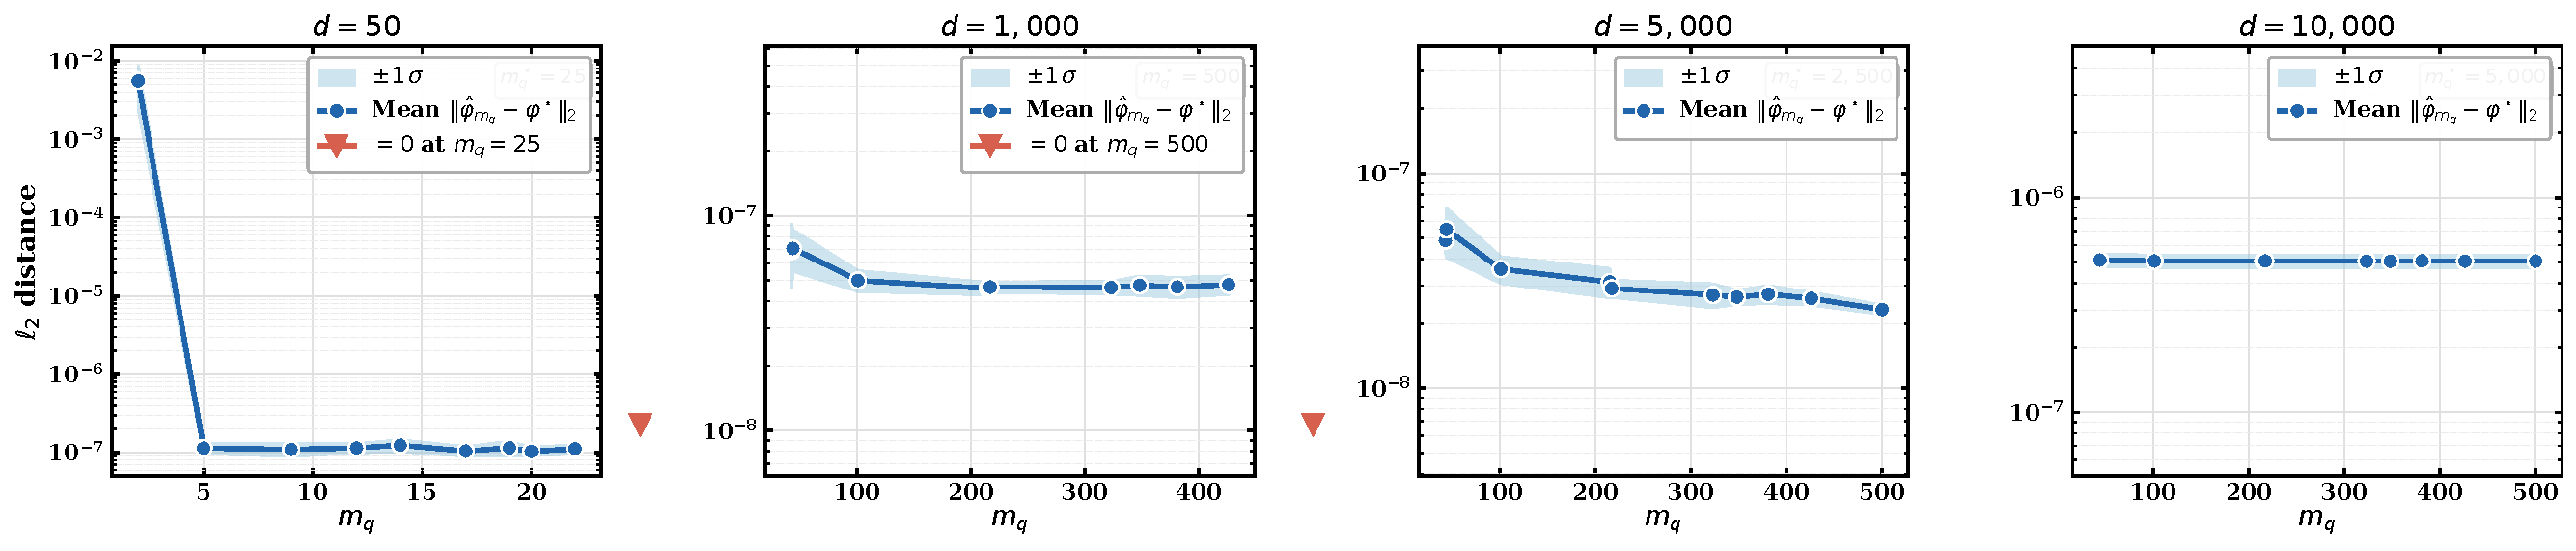
\includegraphics[width=\linewidth]{../benchmarks/results/mq/mq_convergence_combined.pdf}
  \caption{%
    Convergence of the GL Shapley approximation to the exact value
    $\varphi^\star$ (computed at $m_q^\star{=}\lceil d/2\rceil$) for a
    KRR model with an RBF kernel.
    Each panel shows the mean $\ell_2$ distance $\pm 1\sigma$ over ten
    test instances as $m_q$ increases.
    The dashed vertical line marks $m_q^\star$ when it falls within the
    plotted range; otherwise its value is annotated in the top-right
    corner.
    For $d\leq 1000$ the curve reaches zero ({\color[HTML]{D6604D}$\boldsymbol{\triangledown}$})
    at $m_q^\star$, confirming exactness.
    For $d\in\{5000,10000\}$, only $m_q\leq 500$ is shown: the error
    already decreases monotonically and remains below $10^{-7}$.}
  \label{fig:mq_convergence}
\end{figure}

\paragraph{TreeSHAP: runtime and numerical stability.}
We benchmark \textsc{QuadraSHAP} against \textsc{shap}~\citep{shap},
\textsc{FastTreeSHAP v1/v2}~\citep{fast_tree_shap}, \textsc{Linear TreeSHAP}~\citep{linear_treeshap, linear_treeshap_repo} and \textsc{shapiq}~\citep{shapiq} on
\texttt{sklearn} random forests trained on synthetic
\texttt{make\_regression} data. We sweep $d \in \{10, 100\}$ features
and ensemble size from $10$ to $10^5$ leaves. For each configuration we
train three independent forests, explain ten held-out samples, and
report the median single-threaded wall time together with the
worst-case additivity residual $\max_i|\mathbb{E}[f]+\sum_j\phi_j(x_i)-f(x_i)|$.

Table~\ref{tab:treeshap_bench} summarises the results.
Our method (\textsc{QuadraSHAP}, $m_q{=}\lceil D/2\rceil$) is the fastest
numerically correct method at every configuration, outperforming
\textsc{FastTreeSHAP v1} by roughly $2{\times}$ and \textsc{shap} by
$3$--$5{\times}$, with the gap widening as the ensemble grows.
Its additivity residual stays at floating-point precision (${\sim}10^{-13}$)
throughout.
\textsc{Linear TreeSHAP} is competitive on wall time but suffers from
catastrophic numerical breakdown: for $d{=}10$ its additivity residual
grows from $6{\times}10^{-14}$ at 10 leaves to $3{\times}10^{-6}$ at $10^3$
leaves and ${\sim}10$ at $10^4$ leaves, making the reported speedups
meaningless at large ensemble sizes.
The instability worsens with feature width: at $d{=}100$ and $10^5$
leaves the residual reaches $7{\times}10^2$.
\textsc{shapiq} is orders of magnitude slower and times out at $10^5$
leaves for $d{=}10$.

\begin{table}[t]
\centering
\small\setlength{\tabcolsep}{4pt}
\caption{Single-threaded TreeSHAP runtime (ms, median over 3 sklearn \texttt{RandomForestRegressor}s with 10 samples each) and worst-case additivity residual $\max_i|\mathbb{E}[f] + \sum_j \phi_{ij} - f(x_i)|$. Best time in each column is \textbf{bold}. {\color{red}Red} residuals indicate numerical breakdown. Columns are total leaves in the ensemble.}
\label{tab:treeshap_bench}
\begin{tabular}{@{}c@{\hspace{3pt}}lccccccc@{}}
\toprule
$d$ & Method & $10$ & $20$ & $50$ & $100$ & $1\text{k}$ & $10\text{k}$ & $100\text{k}$ \\
\midrule
%% ── d = 10 ──────────────────────────────────────────────────────────────────
\multirow{12}{*}{\rotatebox{90}{\footnotesize\bfseries $d = 10$}}
& \textsc{shap} & 0.009 & 0.017 & 0.037 & 0.089 & 1.1 & 14.3 & 189 \\
& & {\scriptsize $5{\cdot}10^{-14}$} & {\scriptsize $6{\cdot}10^{-14}$} & {\scriptsize $1{\cdot}10^{-13}$} & {\scriptsize $1{\cdot}10^{-13}$} & {\scriptsize $3{\cdot}10^{-13}$} & {\scriptsize $1{\cdot}10^{-12}$} & {\scriptsize $3{\cdot}10^{-12}$} \\[2pt]
& \textsc{FastTreeSHAP v1} & 0.010 & 0.013 & 0.025 & 0.048 & 0.63 & 7.9 & 98.1 \\
& & {\scriptsize $5{\cdot}10^{-14}$} & {\scriptsize $9{\cdot}10^{-14}$} & {\scriptsize $9{\cdot}10^{-14}$} & {\scriptsize $1{\cdot}10^{-13}$} & {\scriptsize $3{\cdot}10^{-13}$} & {\scriptsize $1{\cdot}10^{-12}$} & {\scriptsize $3{\cdot}10^{-12}$} \\[2pt]
& \textsc{FastTreeSHAP v2} & 0.037 & 0.042 & 0.062 & 0.11 & 2.4 & 7.8 & 95.9 \\
& & {\scriptsize $3{\cdot}10^{-14}$} & {\scriptsize $6{\cdot}10^{-14}$} & {\scriptsize $6{\cdot}10^{-14}$} & {\scriptsize $1{\cdot}10^{-13}$} & {\scriptsize $2{\cdot}10^{-13}$} & {\scriptsize $1{\cdot}10^{-12}$} & {\scriptsize $3{\cdot}10^{-12}$} \\[2pt]
& \textsc{linear\_tree\_shap} & 0.014 & 0.019 & 0.029 & 0.048 & 0.49 & 6.3 & 69.0 \\
& & {\scriptsize $6{\cdot}10^{-14}$} & {\scriptsize $2{\cdot}10^{-13}$} & {\scriptsize $8{\cdot}10^{-12}$} & {\scriptsize $9{\cdot}10^{-11}$} & {\scriptsize \textcolor{red}{$3{\cdot}10^{-6}$}} & {\scriptsize \textcolor{red}{$1{\cdot}10^{1}$}} & {\scriptsize \textcolor{red}{$2{\cdot}10^{1}$}} \\[2pt]
& \textsc{shapiq} & 3.3 & 7.8 & 24.3 & 53.5 & 576 & 6198 & timeout \\
& & {\scriptsize $2{\cdot}10^{-13}$} & {\scriptsize $3{\cdot}10^{-13}$} & {\scriptsize $3{\cdot}10^{-13}$} & {\scriptsize $1{\cdot}10^{-12}$} & {\scriptsize $1{\cdot}10^{-11}$} & {\scriptsize $9{\cdot}10^{-11}$} & \\[2pt]
& \textbf{QuadraSHAP} ($m_q{=}\lceil D/2 \rceil$) & \textbf{0.006} & \textbf{0.009} & \textbf{0.017} & \textbf{0.031} & \textbf{0.29} & \textbf{3.8} & \textbf{45.5} \\
& & {\scriptsize $4{\cdot}10^{-14}$} & {\scriptsize $6{\cdot}10^{-14}$} & {\scriptsize $6{\cdot}10^{-14}$} & {\scriptsize $1{\cdot}10^{-13}$} & {\scriptsize $2{\cdot}10^{-13}$} & {\scriptsize $6{\cdot}10^{-13}$} & {\scriptsize $8{\cdot}10^{-13}$} \\[2pt]
\midrule
%% ── d = 100 ─────────────────────────────────────────────────────────────────
\multirow{12}{*}{\rotatebox{90}{\footnotesize\bfseries $d = 100$}}
& \textsc{shap} & 0.011 & 0.017 & 0.039 & 0.099 & 1.3 & 21.6 & 258 \\
& & {\scriptsize $9{\cdot}10^{-14}$} & {\scriptsize $7{\cdot}10^{-14}$} & {\scriptsize $1{\cdot}10^{-13}$} & {\scriptsize $2{\cdot}10^{-13}$} & {\scriptsize $6{\cdot}10^{-13}$} & {\scriptsize $2{\cdot}10^{-12}$} & {\scriptsize $6{\cdot}10^{-12}$} \\[2pt]
& \textsc{FastTreeSHAP v1} & 0.010 & 0.013 & 0.027 & 0.054 & 0.72 & 10.5 & 132 \\
& & {\scriptsize $6{\cdot}10^{-14}$} & {\scriptsize $1{\cdot}10^{-13}$} & {\scriptsize $1{\cdot}10^{-13}$} & {\scriptsize $2{\cdot}10^{-13}$} & {\scriptsize $7{\cdot}10^{-13}$} & {\scriptsize $2{\cdot}10^{-12}$} & {\scriptsize $6{\cdot}10^{-12}$} \\[2pt]
& \textsc{FastTreeSHAP v2} & 0.037 & 0.043 & 0.069 & 0.14 & 3.7 & 10.7 & 120 \\
& & {\scriptsize $6{\cdot}10^{-14}$} & {\scriptsize $6{\cdot}10^{-14}$} & {\scriptsize $6{\cdot}10^{-14}$} & {\scriptsize $2{\cdot}10^{-13}$} & {\scriptsize $6{\cdot}10^{-13}$} & {\scriptsize $2{\cdot}10^{-12}$} & {\scriptsize $6{\cdot}10^{-12}$} \\[2pt]
& \textsc{linear\_tree\_shap} & 0.016 & 0.021 & 0.029 & 0.049 & 0.50 & 6.0 & 65.2 \\
& & {\scriptsize $6{\cdot}10^{-14}$} & {\scriptsize $2{\cdot}10^{-13}$} & {\scriptsize $1{\cdot}10^{-12}$} & {\scriptsize $1{\cdot}10^{-10}$} & {\scriptsize \textcolor{red}{$2{\cdot}10^{-5}$}} & {\scriptsize \textcolor{red}{$6{\cdot}10^{0}$}} & {\scriptsize \textcolor{red}{$7{\cdot}10^{2}$}} \\[2pt]
& \textsc{shapiq} & 3.3 & 6.8 & 21.1 & 46.5 & 580 & 4597 & 45911 \\
& & {\scriptsize $2{\cdot}10^{-13}$} & {\scriptsize $7{\cdot}10^{-14}$} & {\scriptsize $2{\cdot}10^{-12}$} & {\scriptsize $3{\cdot}10^{-12}$} & {\scriptsize $3{\cdot}10^{-9}$} & {\scriptsize $9{\cdot}10^{-5}$} & {\scriptsize $1{\cdot}10^{-4}$} \\[2pt]
& \textbf{QuadraSHAP} ($m_q{=}\lceil D/2 \rceil$) & \textbf{0.006} & \textbf{0.009} & \textbf{0.016} & \textbf{0.030} & \textbf{0.32} & \textbf{4.1} & \textbf{50.4} \\
& & {\scriptsize $6{\cdot}10^{-14}$} & {\scriptsize $6{\cdot}10^{-14}$} & {\scriptsize $2{\cdot}10^{-13}$} & {\scriptsize $1{\cdot}10^{-13}$} & {\scriptsize $2{\cdot}10^{-13}$} & {\scriptsize $4{\cdot}10^{-13}$} & {\scriptsize $5{\cdot}10^{-13}$} \\[2pt]
\bottomrule
\end{tabular}
\end{table}





\appendix



%%%%%%%%%%%%%%%%%%%%%%%%%%%%%%%%%%%%%%%%%%%%%
%%%%% Appendix
%%%%%%%%%%%%%%%%%%%%%%%%%%%%%%%%%%%%%%%%%%%%%
\section{Appendix}
\section{Proofs}\label{apx:proofs}

\subsection*{Proof of Proposition \ref{prop:shapley_integral_identity_product_game}}
% \begin{proof}
By definition, the Shapley value of player $i\in\cD$ is
\[
\phi_i(v)
=
\sum_{S\subseteq \cD\setminus\{i\}}
\frac{|S|!\,(d-|S|-1)!}{d!}
\bigl(v(S\cup\{i\})-v(S)\bigr).
\]
For a product game, the marginal contribution simplifies to
\[
v(S\cup\{i\})-v(S)
=
\Bigl(\prod_{j\in S}u_j\Bigr)(u_i-1).
\]
Substituting this expression yields
\[
\phi_i(v)
=
(u_i-1)
\sum_{S\subseteq \cD\setminus\{i\}}
\mu_{|S|}
\prod_{j\in S}u_j,
\qquad
\mu_q := \frac{q!\,(d-q-1)!}{d!}.
\]

We now express the coefficients $\mu_q$ as integrals. For integers
$q\in\{0,\dots,d-1\}$, consider the integral
\[
\int_0^1 t^q(1-t)^{d-q-1}\,dt.
\]
By repeated integration by parts (or by the definition of the Beta function),
this integral evaluates to
\[
\int_0^1 t^q(1-t)^{d-q-1}\,dt
=
\frac{q!\,(d-q-1)!}{d!}
=
\mu_q.
\]
Thus, each Shapley weight $\mu_q$ admits the representation
\[
\mu_q
=
\int_0^1 t^q(1-t)^{d-q-1}\,dt.
\]

Substituting this identity into the Shapley expression and interchanging
summation and integration gives
\[
\phi_i(v)
=
(u_i-1)
\int_0^1
\sum_{S\subseteq \cD\setminus\{i\}}
t^{|S|}(1-t)^{d-|S|-1}
\prod_{j\in S}u_j
\,dt.
\]

To simplify the inner sum, observe that for each feature $j\neq i$, the term
inside the summation contributes either a factor $(1-t)$ if $j\notin S$ or
a factor $t\,u_j$ if $j\in S$. Summing over all subsets
$S\subseteq \cD\setminus\{i\}$ therefore corresponds to expanding the product
\[
\prod_{j\neq i}\bigl((1-t)+t\,u_j\bigr).
\]
Since $|\cD\setminus\{i\}|=d-1$, this expansion yields
\[
\sum_{S\subseteq \cD\setminus\{i\}}
t^{|S|}(1-t)^{d-|S|-1}\prod_{j\in S}u_j
=
\prod_{j\neq i}\bigl((1-t)+t\,u_j\bigr).
\]

Substituting back into the integral completes the proof:
\[
\phi_i(v)
=
(u_i-1)
\int_0^1
\prod_{j\neq i}\bigl((1-t)+t\,u_j\bigr)\,dt.
\]
% \end{proof}

\subsection*{Proof of Lemma~\ref{lem:gl_shapley_integral}}

\paragraph{Part~(i): Exactness.}
The integrand $g_i(t):=\prod_{j\neq i}\bigl((1-t)+tu_j\bigr)$ is a polynomial
of degree at most $d-1$ in $t$.
An $m_q$-point GL rule on $[0,1]$ integrates exactly every polynomial of degree
at most $2m_q-1$~\citep{davis1984methods}.
For $m_q\ge\lceil d/2\rceil$ we have $2m_q-1\ge 2\lceil d/2\rceil-1\ge d-1$,
so the quadrature sum reproduces the exact integral:
\[
\sum_{q=1}^{m_q}\omega_q\,g_i(\tau_q)
\;=\;
\int_0^1 g_i(t)\,dt.
\]
Multiplying both sides by $(u_i-1)$ and applying
Proposition~\ref{prop:shapley_integral_identity_product_game} gives
$\widehat{\phi}_i(v)=\phi_i(v)$.

\paragraph{Part~(ii): Approximation.}
Let
\[
g_i(t):=\prod_{j\neq i}\bigl((1-t)+t\,u_j\bigr).
\]
By Proposition~\ref{prop:shapley_integral_identity_product_game}, the exact
Shapley value admits the integral representation
\[
\phi_i(v)
=
(u_i-1)\int_0^1 g_i(t)\,dt,
\]
while its \(m_q\)-point Gauss--Legendre approximation is
\[
\widehat{\phi}_i(v)
=
(u_i-1)\sum_{q=1}^{m_q}\omega_q\,g_i(\tau_q).
\]
Therefore,
\[
\bigl|\phi_i(v)-\widehat{\phi}_i(v)\bigr|
=
|u_i-1|
\left|
\int_0^1 g_i(t)\,dt
-
\sum_{q=1}^{m_q}\omega_q\,g_i(\tau_q)
\right|.
\]

Now \(g_i\) is a polynomial in \(t\) of degree at most \(d-1\), hence it is
entire and in particular analytic on and inside every Bernstein ellipse
\(E_\rho\), for any \(\rho>1\). Standard Gauss--Legendre quadrature error
bounds for analytic functions on \([-1,1]\) \citep[Thm.~19.3]{trefethen2013atap},
transferred to \([0,1]\) via the affine change of variables \(x=2t-1\), imply
\[
\left|
\int_0^1 g_i(t)\,dt
-
\sum_{q=1}^{m_q}\omega_q\,g_i(\tau_q)
\right|
\le
\frac{4\max_{z\in E_\rho}|g_i(z)|}{\rho^{2m_q}(\rho^2-1)}.
\]
Substituting this bound into the previous display yields
\[
\bigl|\phi_i(v)-\widehat{\phi}_i(v)\bigr|
\le
|u_i-1|
\frac{4\max_{z\in E_\rho}|g_i(z)|}{\rho^{2m_q}(\rho^2-1)}.
\]
Hence, for any fixed \(\rho>1\),
\[
\bigl|\phi_i(v)-\widehat{\phi}_i(v)\bigr|
\le
C_\rho\,M_\rho\,|u_i-1|\,\rho^{-2m_q},
\]
where $M_\rho:=\max_{z\in E_\rho}|g_i(z)|$ and $C_\rho:=4/(\rho^2-1)$ depends only on $\rho$.
This proves the claimed geometric decay of the approximation error. \qed

\subsection*{Proof of Proposition~\ref{prop:complexity}}

\paragraph{Work.}
Computing, for each $q\in\{1,\dots,m_q\}$, the factors $T_{q,j}=(1-\tau_q)+\tau_q u_j$ and the associated quantities $\log|T_{q,j}|$ and $\mathrm{sgn}(T_{q,j})$ costs $O(d\,m_q)$ arithmetic operations in total. Accumulating $\log|P_q|=\sum_j \log|T_{q,j}|$ and $\mathrm{sgn}(P_q)=\prod_j \mathrm{sgn}(T_{q,j})$ is a length-$d$ reduction for each of the $m_q$ nodes, contributing $O(d\,m_q)$ additional work. Evaluating \cref{eq:gl_logspace_phi} then requires, for each $i\in\{1,\dots,d\}$, a weighted sum of $m_q$ terms, each obtained from $\log|P_q|-\log|T_{q,i}|$ in constant time, for a further $O(d\,m_q)$ operations. The total is therefore $O(d\,m_q)$.

\paragraph{Parallel time.}
Given an associative operator $\oplus$ and a length-$L$ sequence, a hierarchical parallel scan evaluates $a_1\oplus\cdots\oplus a_L$ in parallel time $O(\log L)$ using $O(L)$ processors~\citep{blelloch1990prefix}. Both $\log|P_q|$ (under addition) and $\mathrm{sgn}(P_q)$ (under multiplication) are such reductions over the feature axis of length $d$, and the $m_q$ nodes are independent, so the shared-product phase completes in parallel time $O(\log d)$. For each $i$, evaluating \cref{eq:gl_logspace_phi} requires (i) subtracting $\log|T_{q,i}|$ from $\log|P_q|$ pointwise (parallel time $O(1)$), and (ii) a weighted sum over $q$, which is a length-$m_q$ tree reduction with parallel time $O(\log m_q)$. Since the $d$ Shapley values are independent given $\{(\log|P_q|,\mathrm{sgn}(P_q))\}_{q=1}^{m_q}$, they are evaluated in parallel across $i$ without increasing parallel time. The overall parallel time is therefore $O(\log d+\log m_q)$. The required number of processors is the ratio of total work to parallel time~\citep{brent1974parallel}, giving $O\!\bigl(d\,m_q/(\log d+\log m_q)\bigr)$ processors. The exact regime $m_q=\lceil d/2\rceil$ is a special case.\qed


% \section{Pseudocode for tree algorithms}
\label{app:tree_algorithms}

\begin{algorithm}[t]
\caption{Optimal DFS algorithm}
\label{alg:optimal_dfs}
\begin{algorithmic}[1]
\Require Tree $T$, explained sample $x$, quadrature nodes and weights $\{(\tau_r,\omega_r)\}_{r=1}^{m_q}$
\Ensure Shapley values $\phi_i$

\Statex \textbf{Definitions:} $a_r(q)=1-\tau_r+\tau_r q$, \quad $s_r(q)=\dfrac{q-1}{a_r(q)}$
\Statex \textbf{State along current DFS path:}
\Statex \hspace{\algorithmicindent} $q[j]$: current factor of feature $j$ (default $1$)
\Statex \hspace{\algorithmicindent} $B[r]$: current product value $\left(\prod_{e\text{ on path}} p_e\right)\prod_j a_r(q[j])$

\ForAll{features $i$}
    \State $\phi_i \gets 0$
\EndFor
\ForAll{features $j$}
    \State $q[j] \gets 1$
\EndFor
\For{$r=1$ to $m_q$}
    \State $B[r] \gets 1$
\EndFor

\Function{DFS}{$u$}
    \If{$u$ is a leaf}
        \For{$r=1$ to $m_q$}
            \State $H[r] \gets V_u \cdot B[r]$
        \EndFor
        \State \Return $H$
    \EndIf

    \For{$r=1$ to $m_q$}
        \State $H_{\mathrm{tot}}[r] \gets 0$
    \EndFor

    \ForAll{child edges $e=(u,v)$}
        \State $j \gets f(e)$
        \State $p \gets p_e$
        \State $c \gets c_e(x)$
        \State $q_{\mathrm{old}} \gets q[j]$
        \State $q_{\mathrm{new}} \gets q_{\mathrm{old}} \cdot c$

        \For{$r=1$ to $m_q$}
            \State $B[r] \gets B[r] \cdot p \cdot \dfrac{a_r(q_{\mathrm{new}})}{a_r(q_{\mathrm{old}})}$
        \EndFor
        \State $q[j] \gets q_{\mathrm{new}}$

        \State $H_{\mathrm{child}} \gets \Call{DFS}{v}$

        \For{$r=1$ to $m_q$}
            \State $\Delta \gets s_r(q_{\mathrm{new}}) - s_r(q_{\mathrm{old}})$
            \State $\phi_j \gets \phi_j + \omega_r \, H_{\mathrm{child}}[r] \, \Delta$
            \State $H_{\mathrm{tot}}[r] \gets H_{\mathrm{tot}}[r] + H_{\mathrm{child}}[r]$
        \EndFor

        \State $q[j] \gets q_{\mathrm{old}}$
        \For{$r=1$ to $m_q$}
            \State $B[r] \gets B[r] \big/ \left(p \cdot \dfrac{a_r(q_{\mathrm{new}})}{a_r(q_{\mathrm{old}})}\right)$
        \EndFor
    \EndFor

    \State \Return $H_{\mathrm{tot}}$
\EndFunction

\State \Call{DFS}{$\mathrm{root}(T)$}
\end{algorithmic}
\end{algorithm}

\paragraph{Complexity.}
When DFS moves across an edge, only one $q_j$ changes, so updating the running quantities costs $O(m_q)$.
Each subtree aggregation and Shapley update also costs $O(m_q)$ per edge.
Since every edge is traversed once downward and once upward, the total running time is $O(m_qL)$.

\paragraph{Numerical note.}
As before, the updates for $q$ and $G$ can be carried out in log-space:
store $\log |G_r|$ (and, if needed, $\log |q_j|$), together with sign bits.
Then multiplications/divisions become additions/subtractions of logs.
Zero values should be handled explicitly rather than by taking logarithms, and special care is needed when $a_r(q)=0$.








\bibliographystyle{plainnat}
\bibliography{references}

\end{document}